\begin{tikzpicture}
    % 两个 scope 的区别,仅仅在于各点的名称不同。
    % 所以将绘制代码抽取出来(复用)
    \def\drawtriangle{
        \tkzDefPoints{0/0/B, 3.5/0/C, 2.8/2/A}
        \tkzDrawPolygon(A,B,C)
        \tkzMarkSegment[mark=|](A,B)
        \tkzMarkSegment[mark=||](B,C)
        \tkzMarkSegment[mark=|||](A,C)
    }

    \begin{scope}
        \drawtriangle
        \tkzLabelPoints[above](A)
        \tkzLabelPoints[below](B,C)
    \end{scope}

    \begin{scope}[xshift=4.5cm]
        \drawtriangle
        \tkzLabelPoint[above](A){$A'$}
        \tkzLabelPoint[below](B){$B'$}
        \tkzLabelPoint[below](C){$C'$}
    \end{scope}
\end{tikzpicture}

